\documentclass[11pt]{article}

% --------------------
% PACOTES ESSENCIAIS
% --------------------
\usepackage[utf8]{inputenc}     % Codificação UTF-8
\usepackage[T1]{fontenc}        % Fonte com acentuação
\usepackage[brazil]{babel}      % Idioma português
\usepackage{amsmath, amssymb}   % Símbolos matemáticos
\usepackage{graphicx}           % Inserção de imagens
\usepackage{geometry}           % Margens personalizadas
\usepackage{fancyhdr}           % Cabeçalhos e rodapés
\usepackage{enumitem}           % Listas personalizadas
%\usepackage{physics}            % Notação física e matemática
\usepackage{hyperref}           % Links no PDF
\usepackage{multicol}           % Colunas (opcional)
\usepackage{xcolor}

% --------------------
% CONFIGURAÇÕES
% --------------------
\geometry{a4paper, margin=2.5cm}

\pagestyle{fancy}
\fancyhf{}
\rhead{Estado Plano de Tensões}
\lhead{Caio Magno Mendonça Nicácio}
\cfoot{\thepage}

\setlength{\parskip}{0.5em}
\setlength{\parindent}{0pt}

% --------------------
% INÍCIO DO DOCUMENTO
% --------------------
\begin{document}
	
	\begin{center}
		\Large\textbf{Estado Plano de Tensões} \\
		\normalsize
		Data: \today
	\end{center}
	
	\hrule
	\vspace{1em}
	
	\tableofcontents
	\newpage
	
	\section{Introdução}
	\label{sec:introducao}
	
	O estado plano de tensões é definido como a condição simplificada do estado geral de tensões (Fig. \ref{fig:estado-geral}a) que ocorre quando um dos componentes de tensão, associado à uma direção do corpo, é desprezível em relação aos demais. Considera-se, precisamente, \textbf{estado plano de tensões} e as tensões são insignificantes em um plano específico.
	
	\begin{figure}[h!]
		\begin{minipage}[b]{0.48\textwidth}
			\centering
			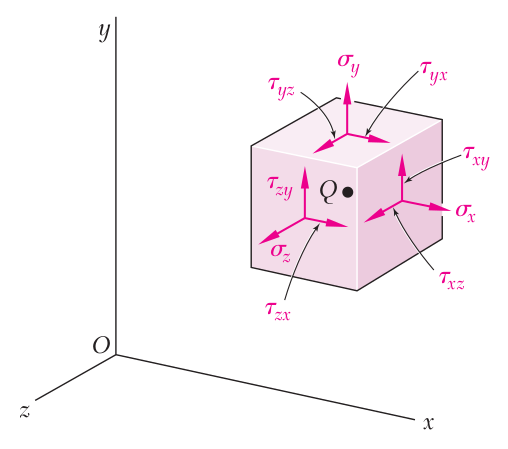
\includegraphics[width=\textwidth]{figure/estado-geral-tensao-1.png}
			\\[-1ex]\small (a)
			\label{fig:estado-geral-1}
		\end{minipage}
		\hfill
		\begin{minipage}[b]{0.48\textwidth}
			\centering
			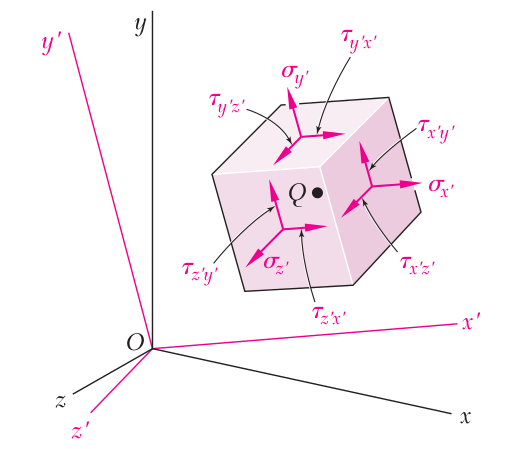
\includegraphics[width=\textwidth]{figure/estado-geral-tensao-2.png}
			\\[-1ex]\small (b)
			\label{fig:estado-geral-2}
		\end{minipage}
		\centering
		%\captionsetup{width=16cm}
		\caption{\centering Representação do estado geral de tensões em um ponto $Q$: (a) no sistema de coordenadas original e (b) no sistema resultante de uma rotação em relação ao sistema inicial.}
		\label{fig:estado-geral}
	\end{figure}

	O estado mais geral de tensões em dado ponto $Q$ pode ser representado pelo \textbf{tensor de tensões de Cauchy}. O mesmo estado poderá ser representado por um conjunto diferente de componentes se os eixos de coordenadas sofrerem rotação (Fig. \ref{fig:estado-geral-2}b).
	\begin{equation}
	\boldsymbol{\sigma} =
	\begin{bmatrix}
		\sigma_{x} & \tau_{xy} & \tau_{xz} \\
		\tau_{yx} & \sigma_{y} & \tau_{yz} \\
		\tau_{zx} & \tau_{zy} & \sigma_{z}
	\end{bmatrix}
	\label{eq:cauchy}
	\end{equation}
	
	O estado geral de tensão é determinado por seis componentes independentes da tensão normal e de cisalhamento. No entanto, não é comum na prática de engenharia a sua aplicação\footnote{Os engenheiros frequentemente fazem simplificações ou aproximações de cargas sobre o corpo, de modo que a tensão produzida em um elemento possa ser analisada em um único plano.}.
	
	Se não houver nenhuma carga em uma superfície de um corpo, as componentes de tensão serão nulas na face de um elemento que estiver na superfície. Por consequência, as tensões na face serão nulas e, portanto, o material no ponto estará sujeito a tensões no plano (Fig. \ref{fig:estado-plano}).
	
	\begin{figure}[h!]
		\centering
		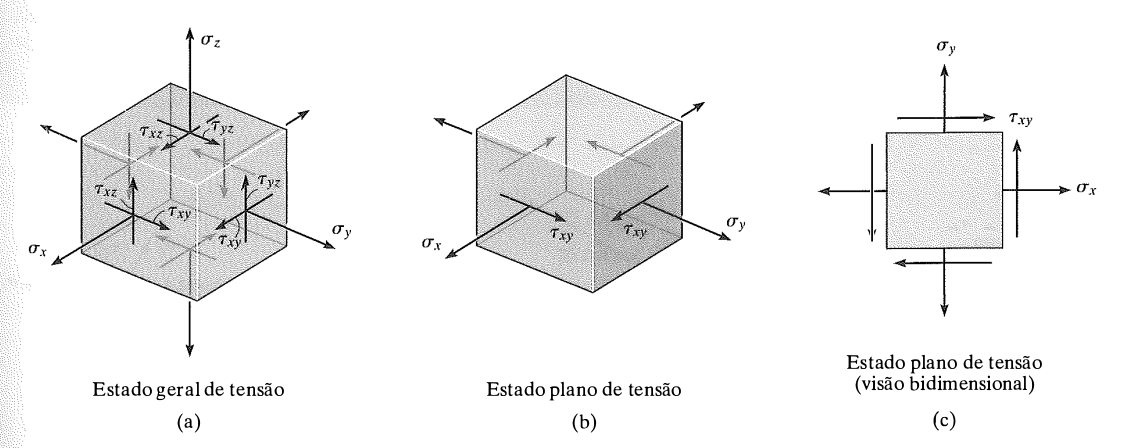
\includegraphics[width=\textwidth]{figure/estado-plano.png}
		%\captionsetup{width=16cm}
		\caption{\centering (a) Representação do estado geral de tensões, (b) do estado plano de tensões e a (c) disposição das tensões ao longo do plano.}
		\label{fig:estado-plano}
	\end{figure}

	Seja $\boldsymbol{\vec{F}}$ uma força aplicada à superfície normal a $\boldsymbol{\vec{n}_z}$. $\sigma_z$, $\tau_{yz}$ e $\tau_{xz}$ são as componentes da tensão na face do elemento diferencial (Fig. \ref{fig:forca-plano-1}). Assumindo que $|\boldsymbol{\vec{F}}|$ é nulo, as componentes de tensão são nulas.
	
	\begin{figure}[h!]
		\centering
		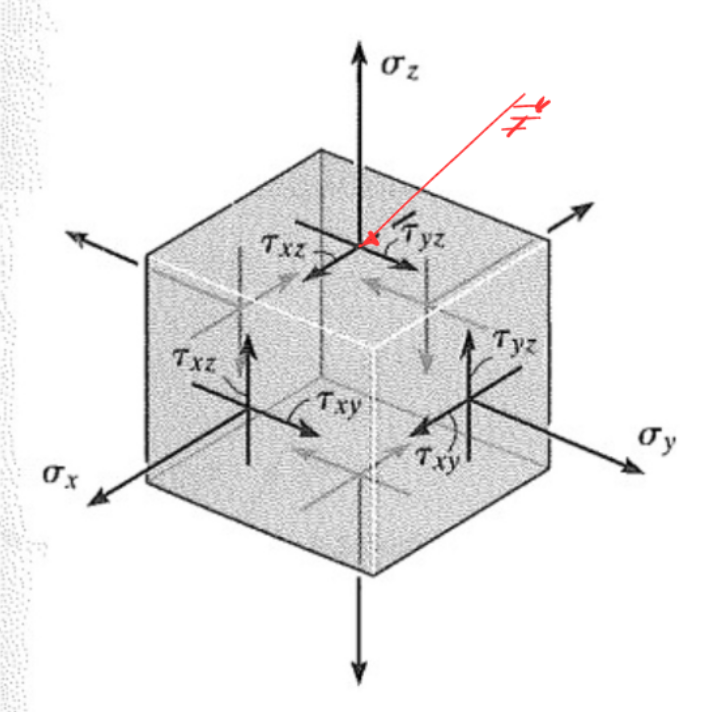
\includegraphics[width=5.5cm]{figure/forca-plano-1.png}
		%\captionsetup{width=16cm}
		\caption{\centering Força $\boldsymbol{\vec{F}}$ aplicada em uma dada superfície.}
		\label{fig:forca-plano-1}
	\end{figure}
	
	As tensões de cisalhamento equilibram o momento em relação ao eixo $z$, de modo que $\sum M_z=0$ (Fig. \ref{fig:equilibrio-momento}).
	\begin{gather*}
		-\tau_{yx}\frac{dy}{2}+\tau_{xy}\frac{dx}{2}=0\\
		\tau_{xy}\, dx=\tau_{yx}\, dy\\
		\boxed{\tau_{xy}=\tau_{yx}},\quad dx\approx dy
	\end{gather*}

	\begin{figure}[h!]
		\centering
		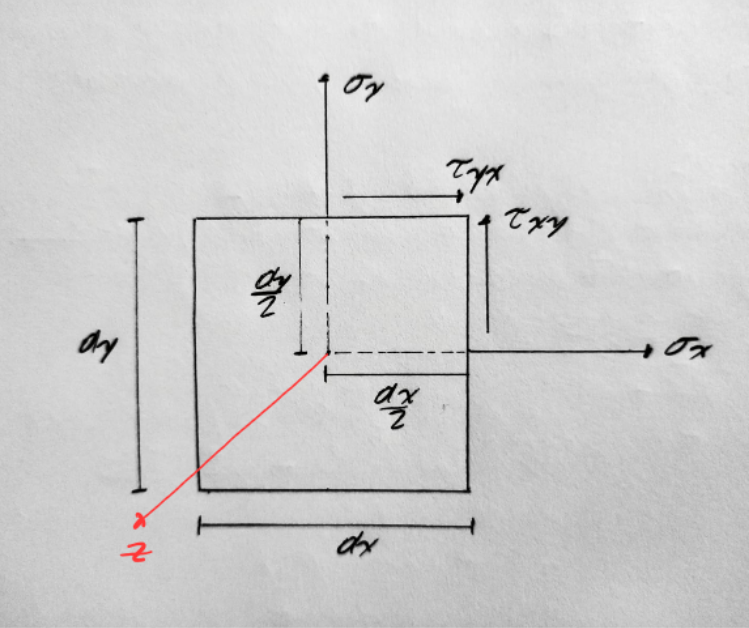
\includegraphics[width=6.5cm]{figure/equilibrio-momento.png}
		%\captionsetup{width=16cm}
		\caption{\centering Estado de tensão no plano normal ao vetor $\boldsymbol{\vec{n}_z}$.}
		\label{fig:equilibrio-momento}
	\end{figure}
	
	O estado geral de tensão no plano e representado por uma combinação de duas componentes de tensão normal, $\sigma_{x}$ e $\sigma_{y}$, e uma componente de tensão de cisalhamento $\tau_{yx}$ que agem nas quatro faces do elemento\footnote{O estado plano de tensão em um ponto é representado exclusivamente por três componentes que agem sobre um elemento de orientação específica neste ponto.}.

	\section{Transformação de tensão}
	\begin{quote}
		\small Transformar as componentes de tensão associadas a um determinado sistema de coordenadas em componentes associadas a um sistema de coordenadas com uma orientação diferente.
	\end{quote}
	
	Uma vez definidas as equações de transformação necessárias, pode-se obter a tensão normal e a tensão de cisalhamento máximas e determinar a orientação do objeto sobre o qual agem.

	\subsection{Transformação de tensão no plano}

	Uma vez que o estado de tensão em um plano é definido por três componentes, então um elemento que tinha orientação diferente está sujeito a três componentes diferentes de tensão (Fig. \ref{fig:estado-plano-2}). Se o estado de tensão for definido pelas componentes $\sigma_{x}$, $\sigma_{y}$ e $\tau_{xy}$, orientadas ao longo dos eixos $x$ e $y$, será possível obter as componentes $\sigma_{x}'$, $\sigma_{y}'$ e $\tau_{xy}'$, orientadas ao longo dos eixos $x'$ e $y'$, que representam o mesmo estado de tensão no ponto\footnote{Quando alterada a orientação, o comportamento é preservado para ambos os sistemas de coordenadas. Isso equivale a conhecer duas componentes $F_x$ e $F_y$, dirigidas ao longo dos eixos $x$ e $y$, que produzem uma força resultante $\boldsymbol{\vec{F}_R}=F_x\mathbf{i}+F_y\mathbf{j}$, e então determinar as componentes $F_x'$ e $F_y'$, que produzem a mesma resultante no sistema de coordenadas orientado pelos eixos $x'$ e $y'$.}.

	\begin{figure}[h!]
		\centering
		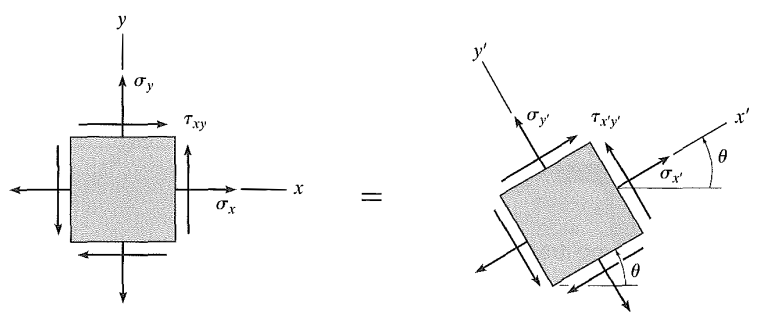
\includegraphics[width=12cm]{figure/estado-plano-2.png}
		%\captionsetup{width=16cm}
		\caption{\centering Transformação do estado plano de tensões.}
		\label{fig:estado-plano-2}
	\end{figure}

	A transformação de componentes de tensão, no entanto, é mais difícil, visto que a transformação deve considerar o valor e a direção de cada componente de tensão e a orientação da área sobre a qual cada componente age. Em um corpo contínuo, quando em equilíbrio estático, as forças internas que atuam sobre os planos obedecem ao \textbf{princípio da transmissibilidade local}\footnote{A resultante das tensões que atuam sobre um plano pode ser transmitida ao plano oposto sem afetar o equilíbrio do elemento diferencial.}.

	\begin{figure}[h!]
		\begin{minipage}[b]{0.48\textwidth}
			\centering
			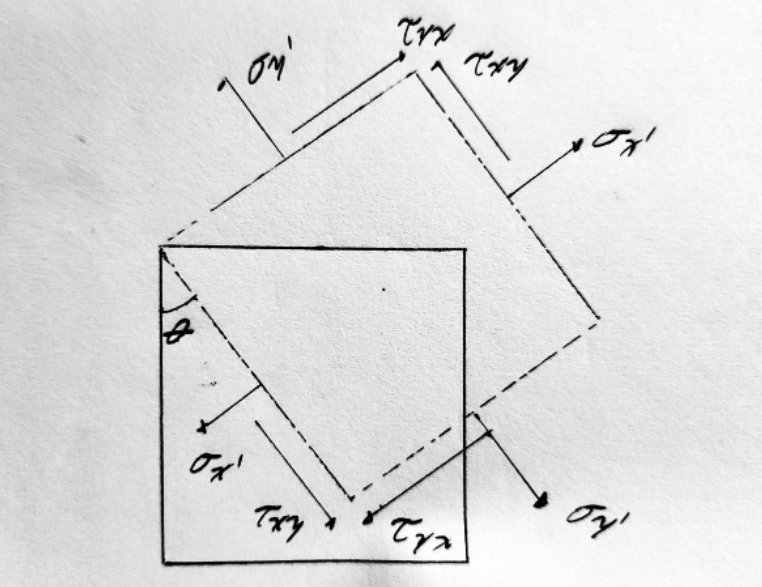
\includegraphics[width=\textwidth]{figure/rotacao.png}
			\\[-1ex]\small (a)
			\label{fig:rotacao}
		\end{minipage}
		\hfill
		\begin{minipage}[b]{0.48\textwidth}
			\centering
			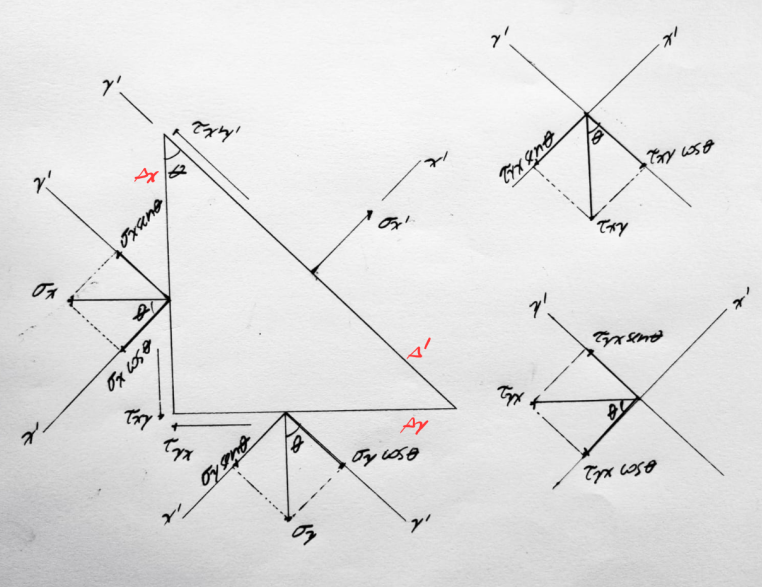
\includegraphics[width=\textwidth]{figure/conversao.png}
			\\[-1ex]\small (b)
			\label{fig:conversao}
		\end{minipage}
		\centering
		%\captionsetup{width=16cm}
		\caption{\centering (a) Tensões no sistema resultante sob rotação e (b) a relação de projeção entre as tensões dos dois sistemas.}
		\label{fig:transformacao-plano}
	\end{figure}
	
	Se o elemento for seccionado por qualquer plano, as tensões que aparecem são projeções do mesmo campo de tensões existente (Fig. \ref{fig:transformacao-plano}).
	
	O somatório das forças é realizado em relação ao plano inclinado, cuja tensão $\sigma_x'$ atua. $A_x=A'\cos \theta$ e $A_y=A'\sin \theta$ são as coordenadas do plano segundo o sistema ortogonal $x'y'$.
	
	Considerando o somatório de forças na direção $x'$, obtêm-se
	\begin{gather*}
		\sum F_x'=0:\qquad \sigma_x'\, A'-\sigma_{x}\,\cos\theta\, A_x-\tau_{xy}\, \cos\theta\, A_y - \tau_{yx}\, \sin\theta\, A_x-\sigma_{y}\,\sin\theta\, A_y=0\\
		\sigma_{x}'\, A'=\sigma_{x}\, A'\, \cos^2 \theta +2\,\tau_{xy}\, A'\,\cos\theta\, \sin\theta-\sigma_{y}\, A'\, \sin^2 \theta\\
		\boxed{\sigma_{x}'=\sigma_{x}\, \cos^2 \theta - \sigma_{y}\, \sin^2 \theta+2\,\tau_{xy}\, \cos\theta\, \sin\theta}.
	\end{gather*}
	A partir do somatório das forças na direção $y'$, conclui-se que
	\begin{gather*}
		\sum F_y'=0:\qquad \tau_{x'y'} \, A'-\tau_{xy}\, \sin\theta \, A_y+\sigma_{x}\, \sin\theta\, A_x-\sigma_{y}\, \cos\theta\, A_y=0\\
		\tau_{x'y'}\, A'=\tau_{xy}\, A'(\cos^2 \theta\, \sin^2 \theta)-(\sigma_{x}-\sigma_{y})\, A'\, \sin \theta\, \cos\theta\\
		\boxed{\tau_{x'y'}=\tau_{xy}\, (\cos^2 \theta - \sin^2 \theta)+(\sigma_{y}-\sigma_{x})\, \sin\theta \, \cos\theta}.
	\end{gather*}
	\textcolor{red}{Fornecer a relação para $\sigma_{y}'$.}
	
	\subsection{Transformação do estado de tensão pela fórmula de Cauchy}
	
	As relações também podem ser derivadas da \textbf{fórmula de Cauchy} para o vetor tração $\boldsymbol{\vec{t}}$.
	\begin{figure}[h!]
		\begin{minipage}[b]{0.48\textwidth}
			\centering
			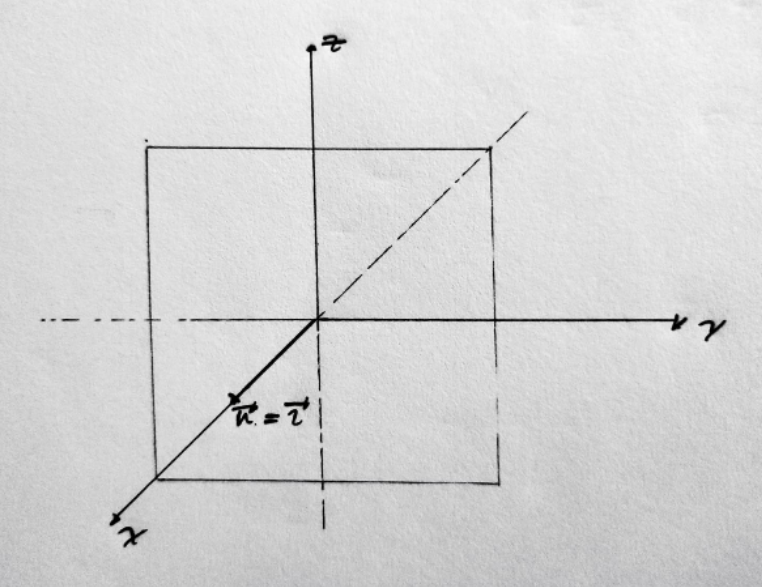
\includegraphics[width=\textwidth]{figure/cauchy-1.png}
			\\[-1ex]\small (a)
			%\label{fig:rotacao}
		\end{minipage}
		\hfill
		\begin{minipage}[b]{0.48\textwidth}
			\centering
			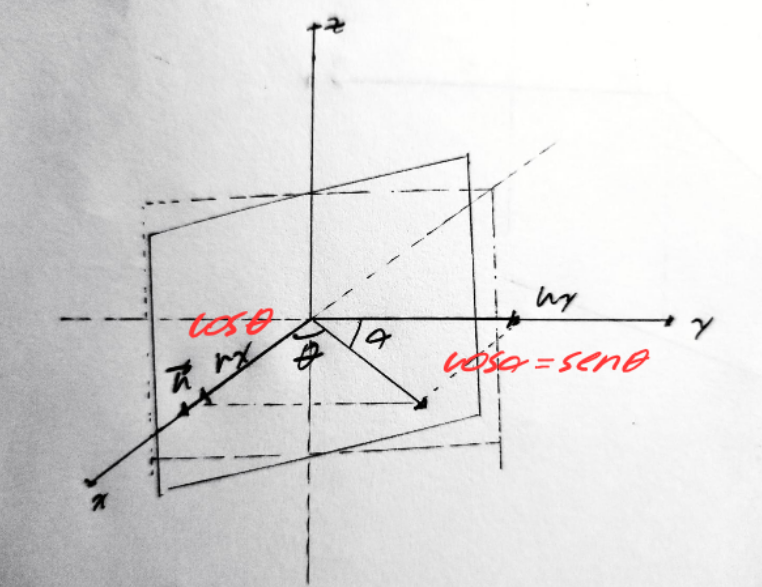
\includegraphics[width=\textwidth]{figure/cauchy-2.png}
			\\[-1ex]\small (b)
			%\label{fig:conversao}
		\end{minipage}
		\centering
		%\captionsetup{width=16cm}
		\caption{\centering (a) Tensões no sistema resultante sob rotação e (b) a relação de projeção entre as tensões dos dois sistemas.}
		\label{fig:rotacao-plano}
	\end{figure}
	Em um estado plano de tensão, o tensor de tensão de Cauchy reduz-se a
	\[
	\boldsymbol{\sigma} =
	\begin{bmatrix}
		\sigma_{x} & \tau_{xy} & 0 \\
		\tau_{yx} & \sigma_{y} & 0 \\
		0 & 0 & 0
	\end{bmatrix}
	=
	\begin{bmatrix}
		\sigma_{x} & \tau_{xy} & 0 \\
		\tau_{xy} & \sigma_{y} & 0 \\
		0 & 0 & 0
	\end{bmatrix}.
	\]
	Para um plano qualquer, o vetor normal unitário é
	\[
	\boldsymbol{\vec{e}_{x'}} =
	\begin{bmatrix}
		n_x \\
		n_y \\
		n_z
	\end{bmatrix}
	=
	\begin{bmatrix}
		\cos \theta \\
		\sin \theta \\
		0
	\end{bmatrix},
	\]
	onde $\theta$ é o ângulo entre $\vec{n}$ e o eixo x, orientado em $\vec{n}_x$.
	
	Como o eixo $x'$ é orientado ortogonalmente a $y'$,
	\[
	\boldsymbol{\vec{e}_{y'}} =
	\begin{bmatrix}
		-\sin \theta \\
		\cos \theta \\
		0
	\end{bmatrix},\quad \boldsymbol{\vec{e}_{x'}}\cdot \boldsymbol{\vec{e}_{y'}}=0.
	\]
	
	A \textbf{matriz de rotação} $\mathbf{R}$ permite rotacionar um vetor em relação a um sistema ortogonal de coordenadas, ao redor do eixo z.
	\[
	\mathbf{R} =
	\begin{bmatrix}
		\boldsymbol{\vec{e}_{x'}} \\
		\boldsymbol{\vec{e}_{y'}} \\
		\boldsymbol{\vec{e}_{z'}}
	\end{bmatrix}^T
	=
	\begin{bmatrix}
		\cos\theta & -\sin\theta & 0 \\
		\sin\theta & \cos\theta & 0 \\
		0 & 0 & 1
	\end{bmatrix}.
	\]
	A matriz $\mathbf{R}$ representa a transformação do sistema de coordenadas. A transformada de tensores de $\sigma$ para $\sigma'$ associado a um novo sistema de coordenadas é dada por
	\[
		\sigma' = \mathbf{R}^T\, \sigma\, \mathbf{R},
	\]
	onde $\sigma'$ é o tensor de tensão do sistema rotacionado.
	
	\subsubsection{Componentes no plano $x'y'$}
	
	$\sigma_{x}'$ é a componente normal no plano ao vetor $\boldsymbol{\vec{e}_{x'}}$.
	\begin{gather*}
	\boldsymbol{\vec{t}_{x'}} = \mathbf{\sigma}\cdot \boldsymbol{\vec{e}_{x'}} =
	\begin{bmatrix}
		\sigma_{x} & \tau_{xy} & 0 \\
		\tau_{yx} & \sigma_{y} & 0 \\
		0 & 0 & 0
	\end{bmatrix}
	\cdot
	\begin{pmatrix}
		\cos \theta \\
		\sin \theta \\
		0
	\end{pmatrix} \\
	\boldsymbol{\vec{t}_{x'}} =
	\begin{pmatrix}
		\sigma_{x}\, \cos \theta + \tau_{xy}\, \sin \theta \\
		\tau_{yx}\, \cos \theta + \sigma_{y}\, \sin \theta \\
		0
	\end{pmatrix}
	\end{gather*}

	A componente normal $\sigma_{x'}$ e a projeção de $\boldsymbol{\vec{t}_{x´}}$ na direção $\boldsymbol{\vec{e}_{x´}}$. Logo,
	\begin{align*}
		\sigma_{x'}&=\boldsymbol{\vec{t}_{x´}}\cdot \boldsymbol{\vec{e}_{x´}} \\
		&=\sigma_{x}\, \cos^2 \theta + \tau_{xy}\, \sin\theta\, \cos\theta + \sigma_{y}\, \sin^2 \theta + \tau_{yx}\, \sin\theta\, \cos\theta + \sigma_{y}\, \sin^2 \theta \\
		\sigma_{x'}&=\sigma_{x}\, \cos^2 \theta + \sigma_{y}\, \sin^2 \theta + 2\, \tau_{xy}\, \sin\theta\, \cos\theta.
	\end{align*}

	$\sigma_{y'}$ é a componente normal no plano ao vetor $\boldsymbol{\vec{e}_{y'}}$.
	\begin{gather*}
		\boldsymbol{\vec{t}_{y'}} = \mathbf{\sigma}\cdot \boldsymbol{\vec{e}_{y'}} =
		\begin{bmatrix}
			\sigma_{x} & \tau_{xy} & 0 \\
			\tau_{yx} & \sigma_{y} & 0 \\
			0 & 0 & 0
		\end{bmatrix}
		\cdot
		\begin{pmatrix}
			-\sin \theta \\
			\cos \theta \\
			0
		\end{pmatrix} \\
		\boldsymbol{\vec{t}_{y'}} =
		\begin{pmatrix}
			-\sigma_{x}\, \sin\theta + \tau_{xy}\, \cos\theta \\
			-\tau_{yx}\, \sin \theta + \sigma_{y}\, \cos \theta \\
			0
		\end{pmatrix}
	\end{gather*}

	A componente normal $\sigma_{y'}$ é a projeção do vetor $\boldsymbol{\vec{t}_{y'}}$ na direção $\boldsymbol{\vec{e}_{y'}}$. Logo,
	\begin{align*}
		\sigma_{y'} &=\boldsymbol{\vec{t}_{y´}}\cdot \boldsymbol{\vec{e}_{y´}}\\
		&=\sigma_{x}\, \sin^2 \theta - \tau_{xy}\, \sin\theta\, \cos\theta - \tau_{xy}\, \cos\theta \, \sin\theta + \sigma_{y}\, \cos^2 \\
		\sigma_{y'}&=\sigma_{x}\, \sin^2 \theta + \sigma_{y}\, \cos^2 \theta - 2\, \tau_{xy}\, \sin\theta\, \cos\theta.
	\end{align*}

	Por sua vez, $\tau_{x'y'}$ é a componente de cisalhamento no plano normal a $\boldsymbol{\vec{e}_{x'}}$, na qual é a projeção de $\boldsymbol{\vec{t}_{x'}}$ na direção $\boldsymbol{\vec{e}_{y'}}$.
	\begin{align*}
		\tau_{x'y'} &=\boldsymbol{\vec{t}_{x'}}\cdot \boldsymbol{\vec{e}_{y'}}\\
		&= - \sigma_{x}\, \cos\theta\, \sin\theta - \tau_{xy}\, \sin^2 \theta + \tau_{xy}\, \cos^2 \theta + \sigma_{y}\, \sin\theta\, \cos\theta \\
		\tau_{x'y'}&=(\sigma_{y}-\sigma_{x})\, \sin\theta\, \cos\theta + \tau_{xy}\, (\cos^2 \theta - \sin^2 \theta).
	\end{align*}
	O produto escalar $\boldsymbol{\vec{t}_{y'}}\cdot \boldsymbol{\vec{e}_{x'}}$ conduz ao mesmo resultado para $\tau_{x'y'}$.
	
	\subsubsection{Demonstração da transformada do tensor de Cauchy}
	
	Seja $\boldsymbol{\vec{v}}$ um vetor arbitrário. A matriz de rotação $\mathbf{R}$ pode ser usada duas finalidades distintas:
	\begin{enumerate}
		\item Rotacionar o vetor relativo ao sistema original de coordenadas (Fig. \ref{fig:coordinate-rotation}a).
		\[
		\boldsymbol{\vec{v}}'=\mathbf{R}\cdot \boldsymbol{\vec{v}}
		\]
		\item Rotacionar o sistema de coordenadas (Fig. \ref{fig:coordinate-rotation}b).
		\[
		\boldsymbol{\vec{v}}'=\mathbf{R}^T\cdot \boldsymbol{\vec{v}}
		\]
	\end{enumerate}

	\begin{figure}[h!]
		\begin{minipage}[b]{0.48\textwidth}
			\centering
			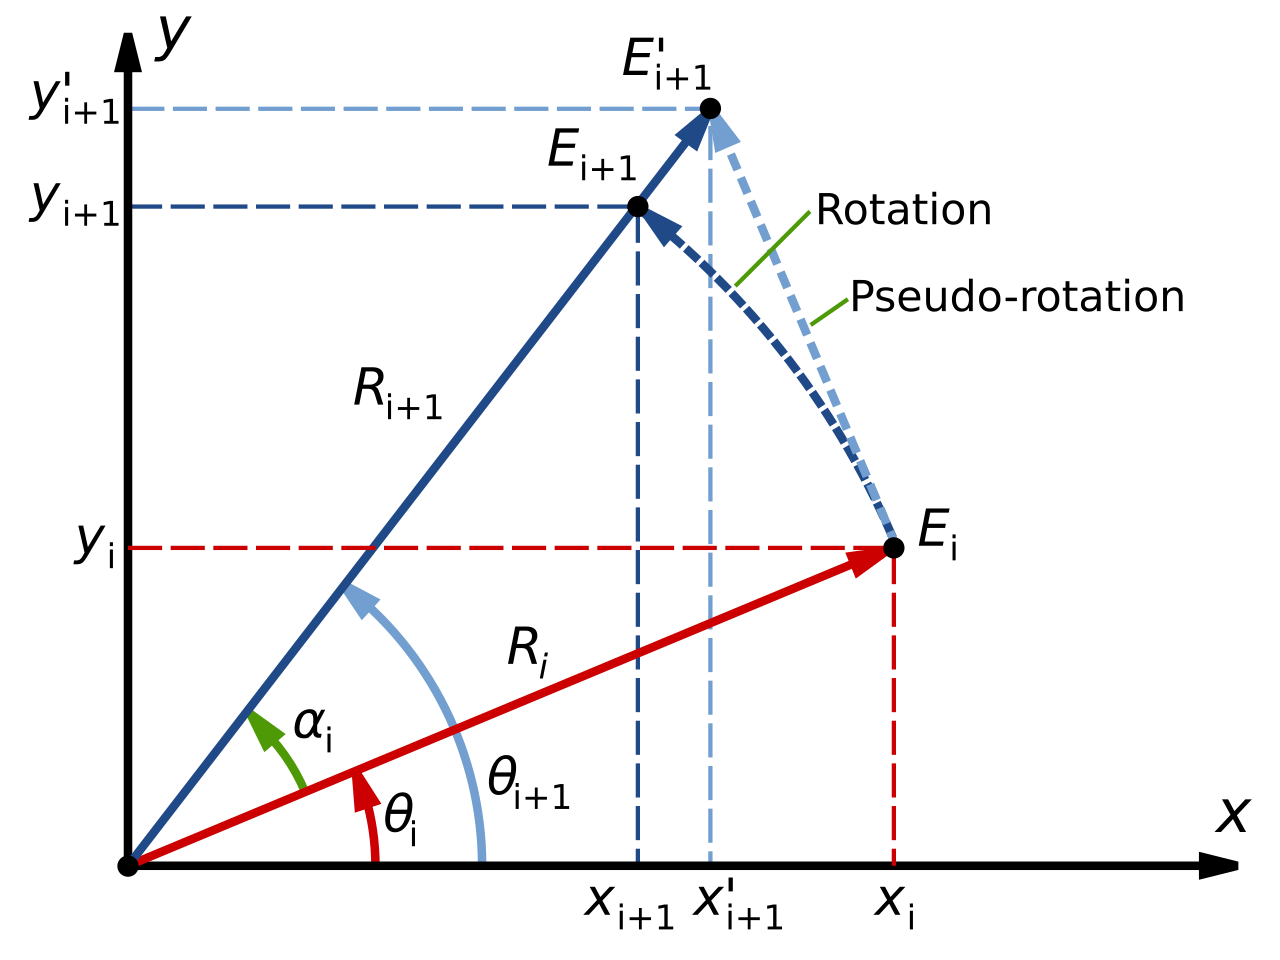
\includegraphics[width=\textwidth]{figure/vector-rotation.png}
			\\[-1ex]\small (a)
		\end{minipage}
		\hfill
		\begin{minipage}[b]{0.48\textwidth}
			\centering
			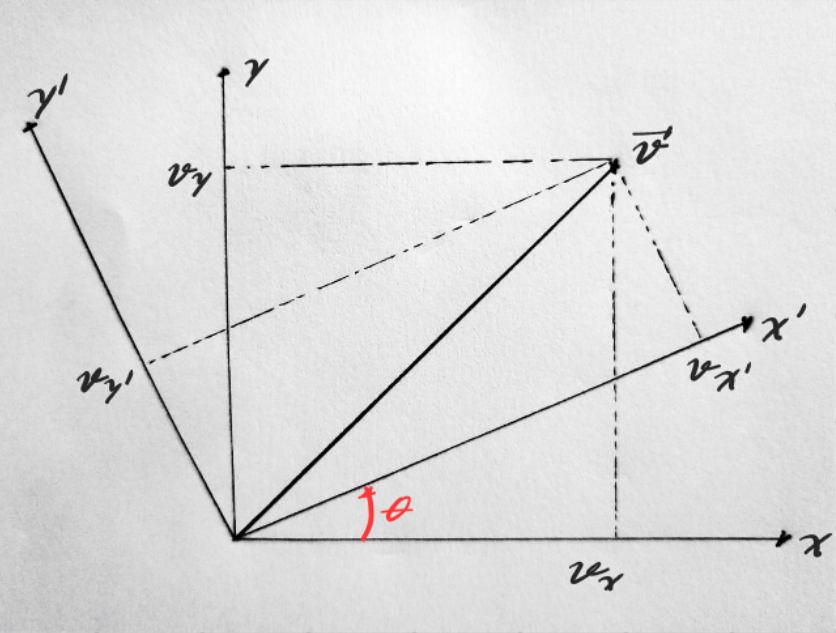
\includegraphics[width=\textwidth]{figure/system-rotation.png}
			\\[-1ex]\small (b)
		\end{minipage}
		\centering
		%\captionsetup{width=16cm}
		\caption{\centering (a) Rotação do vetor, relativo ao sistema ortogonal, e (b) rotação do sistema de coordenadas.}
		\label{fig:coordinate-rotation}
	\end{figure}

	Na análise de tensões, tratam-se a transformação do sistema de coordenadas.
	\[
	\mathbf{\sigma}'=\mathbf{R}^T\, \mathbf{\sigma}\, \mathbf{R}
	\]
	$\mathbf{\sigma}'$ representa o mesmo estado físico de tensão, mas expresso em termos de outro sistema de coordenadas.
	Sabe-se que, para qualquer plano com normal $\boldsymbol{\vec{n}}$,
	\[
	\boldsymbol{\vec{t}}=\mathbf{\sigma}\cdot \boldsymbol{\vec{n}}, \quad \boldsymbol{\vec{t}}'=\mathbf{\sigma}'\cdot \boldsymbol{\vec{n}}'.
	\]
	Os mesmo vetores físicos $\boldsymbol{\vec{t}}$ e $\boldsymbol{\vec{n}}$ se relacionam por
	\[
	\boldsymbol{\vec{t}}'=\mathbf{R}^T\cdot \boldsymbol{\vec{t}}, \quad \boldsymbol{\vec{n}}'=\mathbf{R}^T\cdot \boldsymbol{\vec{n}}.
	\]
	Fazendo a substituição,
	\begin{align*}
	\boldsymbol{\vec{t}}'&=\mathbf{\sigma}\cdot \boldsymbol{\vec{n}}' \\
	\mathbf{R}^T\,(\mathbf{\sigma}\cdot \boldsymbol{\vec{n}}) &= \mathbf{\sigma}'(\mathbf{R}^T\cdot \boldsymbol{\vec{n}}).
	\end{align*}
	Para qualquer $\boldsymbol{\vec{n}}$, temos
	\[
	\mathbf{R}^T\, \mathbf{\sigma}=\mathbf{\sigma}'\, \mathbf{R}^T.
	\]
	Multiplicando ambos os lados por $\mathbf{R}$, é possível obter
	\begin{gather*}
	\mathbf{R}^T\, \mathbf{\sigma}\, \mathbf{R}=\mathbf{\sigma}'\, \mathbf{R}^T\, \mathbf{R} \\
	\boxed{\mathbf{\sigma}'=\mathbf{R}^T\, \mathbf{\sigma}\, \mathbf{R}}, \quad \mathbf{R}^T\, \mathbf{R}=\mathbf{I}.
	\end{gather*}

	\section{Vetor tração e fórmula de Cauchy}
	
	A \textbf{força interna resultante} $\mathbf{T}^{(n)}$ pode ser calculada, quando selecionado um elemento estrutural. Seleciona-se um ponto $P$ na qual irá passar o plano de corte, com orientação segundo um versor $\boldsymbol{\vec{n}}$ (Fig. \ref{fig:stress-vector}).
	\begin{figure}[h!]
		\centering
		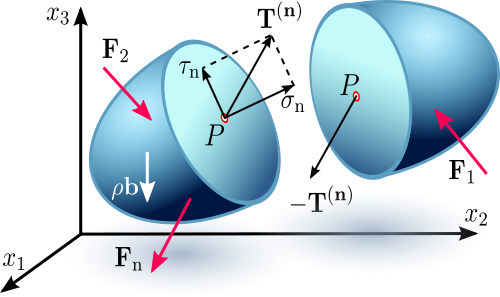
\includegraphics[width=8cm]{figure/stress-vector.png}
		%\captionsetup{width=16cm}
		\caption{\centering Força interna resultante $\mathbf{T}^{(n)}$ de uma seção com orientação arbitrária.}
		\label{fig:stress-vector}
	\end{figure}

	Por definição, $\mathbf{T}^{(n)}=\lim_{\Delta A \to 0}\frac{\sum \boldsymbol{\vec{F}}}{\Delta A}$. Visto que $\sum \boldsymbol{\vec{F}}$ é uma grandeza vetorial, tal que 
	\[
	\sum \boldsymbol{\vec{F}}=\Delta F\,\mathbf{n}+\Delta V_s\, \mathbf{s}+\Delta V_t\, \mathbf{t},
	\]
	pode-se concluir que
	\begin{gather*}
	\mathbf{T}^{(n)}=\lim_{\Delta A \to 0} \left(\frac{\Delta F}{\Delta A}\, \mathbf{n}+\frac{\Delta V_s}{\Delta A}\, \mathbf{s}+\frac{\Delta V_t}{\Delta A}\, \mathbf{t}\right) \\
	\mathbf{T}^{(n)}=\sigma_n\, \mathbf{n}+\tau_{ns}\, \mathbf{s}+\tau_{nt}\, \mathbf{t},
	\end{gather*}
	onde $\tau_{ns}$ e $\tau_{nt}$ representam as componentes da tensão de cisalhamento $\tau_{n}$ no plano ortogonal $st$ da superfície selecionada.
	
	O estado geral de tensões ao redor de um ponto é dado pelo tensor de tensões de Cauchy (Eq. \ref{eq:cauchy}), que descreve o estado de tensões em relação aos planos perpendiculares aos eixos do sistema cartesiano de três dimensões (Fig. \ref{fig:stress-system}).
	
	\begin{figure}[h!]
		\centering
		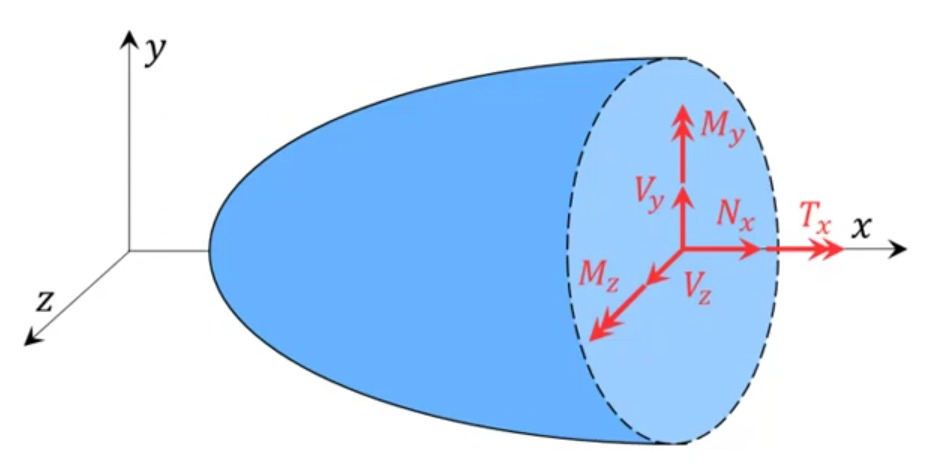
\includegraphics[width=8cm]{figure/stress-system.jpeg}
		%\captionsetup{width=16cm}
		\caption{\centering Estado de tensão em um plano perpendicular ao eixo $x$ do sistema cartesiano.}
		\label{fig:stress-system}
	\end{figure}

	O tensor $\mathbf{\sigma}$  é uma forma sistemática e compacta de representar todas as componentes de tensão que atuam sobre um ponto material em um corpo contínuo, considerado todos os três plano ortogonais associados ao sistema cartesiano. Um estado mais geral de tensão pode ser completamente representado por seis componentes independentes, tal que
	\begin{gather*}
		\mathbf{\sigma} =
		\begin{bmatrix}
			\sigma_{x} & \tau_{xy} & \tau_{xz} \\
			\tau_{yx} & \sigma_{y} & \tau_{yz} \\
			\tau_{zx} & \tau_{zy} & \sigma_{z}
		\end{bmatrix}
		=
		\begin{bmatrix}
			\sigma_{x} & \tau_{yx} & \tau_{zx} \\
			\tau_{xy} & \sigma_{y} & \tau_{zy} \\
			\tau_{xz} & \tau_{yz} & \sigma_{z}
		\end{bmatrix}
		=
		\mathbf{\sigma}^T.
	\end{gather*}
	
	Seja $\boldsymbol{\vec{n}}$ o vetor normal a um plano arbitrário com coordenadas segundo o sistema ortogonal cartesiano, obtêm-se o vetor de tensão $\boldsymbol{\vec{t}}$ que representa a resultante das tensões normal e de cisalhamento. A Equação \ref{eq:cauchy-equation} é denominada \textbf{fórmula de Cauchy}.
	\begin{equation}
		\boldsymbol{\vec{t}} = \mathbf{\sigma}\cdot \boldsymbol{\vec{n}} =
		\begin{bmatrix}
			\sigma_{x} & \tau_{xy} & \tau_{xz} \\
			\tau_{yx} & \sigma_{y} & \tau_{yz} \\
			\tau_{zx} & \tau_{zy} & \sigma_{z}
		\end{bmatrix}
		\cdot
		\begin{pmatrix}
			n_x \\
			n_y \\
			n_z
		\end{pmatrix}
		\label{eq:cauchy-equation}
	\end{equation}
	Genericamente, obtemos
	\[
	\boldsymbol{\vec{t}} =
	\begin{bmatrix}
		t_x \\
		t_y \\
		t_z
	\end{bmatrix}
	=
	\begin{bmatrix}
		\sigma_{x}\, n_x+\tau_{yx}\, n_y+\tau_{zx}\, n_z \\
		\tau_{xy}\, n_x+\sigma_{y}\, n_y+\tau_{zy}\, n_z \\
		\tau_{xz}\, n_x+\tau_{yz}\, n_y+\sigma_{z}\, n_z
	\end{bmatrix}.
	\]
	
	Visto que $\tau_{ij}=\tau_{ji}$,
	\[
	\boldsymbol{\vec{t}} =
	\begin{bmatrix}
		t_x \\
		t_y \\
		t_z
	\end{bmatrix}
	=
	\begin{bmatrix}
		\sigma_{x}\, n_x+\tau_{xy}\, n_y+\tau_{xz}\, n_z \\
		\tau_{yx}\, n_x+\sigma_{y}\, n_y+\tau_{yz}\, n_z \\
		\tau_{zy}\, n_x+\tau_{zy}\, n_y+\sigma_{z}\, n_z
	\end{bmatrix},
	\]
	onde $t_x$, $t_y$ e $t_z$ são as componentes cartesianas do vetor tensão resultante $\boldsymbol{\vec{t}}$, onde cada linha é um escalar aplicado ao plano com normal $\boldsymbol{\vec{n}}$.
	
	%\bibliography{pos-textuais/referencias.bib}

\end{document}